%!TEX root = ../thesis.tex

\thispagestyle{myheadings}

\graphicspath{{Body/Figures/ExperimentalOverview/Decay/}{Body/Figures/TrackingFigures/TrackerPics/}{Body/Figures/ExperimentalOverview/Ring/}{Body/Figures/ExperimentalOverview/Auxiliary/}{Body/Figures/MagneticField/}}

\chapter{Principle Technique of E989}
\label{chapter:E989}

As referenced in \equref{eq:torque}, a particle in a magnetic field will experience a torque which attempts to line up the magnetic dipole moment of the particle with the external field. Because of this, in a dipole field a particles spin will turn at the Larmour precesssion frequency \cite{Jackson}
        \begin{align} \label{eq:ws}
            \vec{\omega}_{s} = -g\frac{q}{2m}\vec{B} - (1-\gamma)\frac{q}{\gamma m}\vec{B},
        \end{align}
where as before $m$ is the particles mass, $q = \pm e$ where $e$ is the elementary charge, \g is the g-factor, $\gamma$ is the Lorentz relativistic factor, and $B$ is an external magnetic field. The second term is a relativistic correction to the precession frequency called Thomas precession \cite{Jackson}. Similarly, a particle with some momentum will orbit at the cyclotron frequency
        \begin{align} \label{eq:wc}
            \vec{\omega}_{c} = -\frac{q}{\gamma m}\vec{B}.
        \end{align}
By taking the difference between these two frequencies we arrive at the "spin difference frequency"
        \begin{align} \label{eq:wasimple}
            \vec{\omega}_{a} = \vec{\omega}_{s} - \vec{\omega}_{c} = -\frac{g-2}{2}\frac{q}{m}\vec{B} = - a \frac{q}{m}\vec{B},
        \end{align}
a frequency that is directly proportional to the anomalous magnetic moment $a$. Briefly note that if $g = 2$ as in a Dirac theory, then the particles spin would turn at the same rate as the momentum vector, and this spin difference frequency \wa would be identically 0. If this spin difference frequency for a muon and the external magnetic dipole field can be measured, then the anomalous magnetic moment of the muon \amu can be measured. 

As will be detailed below in \secref{sec:BIntro}, the measurement of the magnetic field is related to the Larmour precession frequency of free protons in water 
        \begin{align} \label{eq:wp}
            \omega_{p} = -g_{p} \frac{e}{2m_{p}} B,
        \end{align}
where $g_{p}$ and $m_{p}$ are the g-factor and mass of the proton respectively. Replacing $B$ and solving for \amu, we arrive at 
        \begin{align} \label{eq:amu}
            a_{\mu} = \frac{g_{p}}{2} \frac{\omega_{a}}{\omega_{p}} \frac{m_{\mu}}{m_{p}}.
        \end{align}
Using the magnetic moment formulas for the proton, electron, and muon as shown in \equref{eq:magneticmoment}, \equref{eq:amu} can be transformed to either of the following cosistent equations:
        \begin{equation} 
        \begin{aligned} \label{eq:amuratios}
            a_{\mu} &= \frac{g_{e}}{2} \frac{\omega_{a}}{\omega_{p}} \frac{m_{\mu}}{m_{e}} \frac{\mu_{p}}{\mu_{e}} \\ 
            a_{\mu} &= \frac{\omega_{a}/\omega_{p}}{\lambda - \omega_{a}/\omega_{p}}
        \end{aligned}
        \end{equation}
Here the $p$, $e$, and $\mu$ subscripts stand for the relevant quanties for the proton, electron, and muon respectively. In the second quation $\lambda = \mu_{\mu}/\mu_{p}$. As mentioned before the electron g-factor $g_{e}$ has been measured to extremely high precision, 0.26 ppt \cite{ElectronMDM,CODATA}. The muon-electron mass ratio $m_{\mu}/m_{e}$ and muon-proton magnetic moment ratio $\lambda$ have been measured to 22 ppb \cite{CODATA,MuoniumHyperfine}. Finally the proton-electron magnetic moment ratio $\mu_{p}/\mu_{e}$ has been measured to 3 ppb \cite{CODATA}. The errors on these terms are small compared to the target uncertainty for E989 of 140 ppb, the measurement of which now comes down to measuring the ratio $\omega_{a}/\omega_{p}$. 


\section{Measuring \texorpdfstring{\wa}{wa}}
\label{section:WaIntro}

How can \wa for muons be measured? The answer lies with two key points in the dynamics of muon decay. Positive muons decay to a positron and two neutrinos, as shown in \figref{fig:mudecay}. The first point is that because of the parity violating nature of the weak interaction, the decay positron will be preferentially emitted right-handed, with its spin directed in the same direction as its momentum \cite{Bucksbaum}. The second key point is that angular momentum must be conserved. Consider the most extreme examples of maximum and minimum energy positrons as shown in \figref{fig:MuonDecayImproved}. In the muon rest frame, decay positrons with maximum energy will be emitted opposite to the two neutrinos. Since neutrinos and anti-neutrinos must be left and right-handed respectively, thus having their spins anti-parallel and parallel to their momentum, by the law of conservation of angular momentum the positron must have its spin be parallel to the spin of the muon at the time of the decay. By the opposite argument, decay positrons emitted with minimum energy such that the neutrinos are ejected opposite to one another must have their spins be anti-parallel to that of the muon at the time of decay. These two points combined together means that higher energy decay postrons will preferentially be emitted in directions parallel to the muon spin at the time of decay, while lower energy decay positrons will preferentially be emitted in directions anti-parallel to the muon spin at the time of the decay. 

\begin{figure}[]
\centering
    \subcaptionbox{$\mu^{+}$ decay through a $W^{+}$ boson to a positron, muon anti-neutrino, and an electron neutrino. This is the dominant decay mode.
    \label{fig:mudecay}}
    {
    \centering
        \begin{tikzpicture}[baseline=(o.base)]
        \begin{feynhand}
        \large
        \setlength{\feynhandlinesize}{1pt}
        \vertex [dot] (o) at (0,0);
        \vertex (a) at (-2,0) {$\mu^{+}$}; 
        \vertex (b) at (1.5,1.5) {$\overline \nu_{\mu}$}; 
        \vertex (c) at (1.5,-1.5);
        \vertex (d) at (3,0) {$\nu_{e}$};
        \vertex (e) at (3,-3) {$e^{+}$};
        \propag [anti fermion] (a) to (o);
        \propag [fermion] (b) to (o);
        \propag [boson] (o) to [edge label' = $W^{+}$] (c);
        \propag [fermion] (c) to (d);
        \propag [anti fermion] (c) to (e);
        \end{feynhand}
        \end{tikzpicture} 
    }
    \hspace{10mm}
    \subcaptionbox{$\pi^{+}$ decay through a $W^{+}$ boson to a $\mu^{+}$.
    \label{fig:pidecay}}
    {
    \centering
        \begin{tikzpicture}[baseline=(o.base)]
        \begin{feynhand}
        \large
        \setlength{\feynhandlinesize}{1pt}
        \vertex [dot] (o) at (0,0);
        \vertex (a) at (-1.5,1.5) {$u$}; 
        \vertex (b) at (-1.5,-1.5) {$\overline d$}; 
        \vertex (c) at (2,0);
        \vertex (d) at (3.5,1.5) {$\mu^{+}$};
        \vertex (e) at (3.5,-1.5) {$\nu_{\mu}$};
        \propag [fermion] (a) to (o);
        \propag [anti fermion] (b) to (o);
        \propag [boson] (o) to [edge label = $W^{+}$] (c);
        \propag [anti fermion] (c) to (d);
        \propag [fermion] (c) to (e);
        \end{feynhand}
        \end{tikzpicture}  
    }
\caption[Feynman diagrams for muon and pion decay]{Feynman diagrams for muon (left) and pion (right) decay.}    
\label{fig:DecayDiagrams}
\end{figure}

\begin{figure}[]
    \centering
    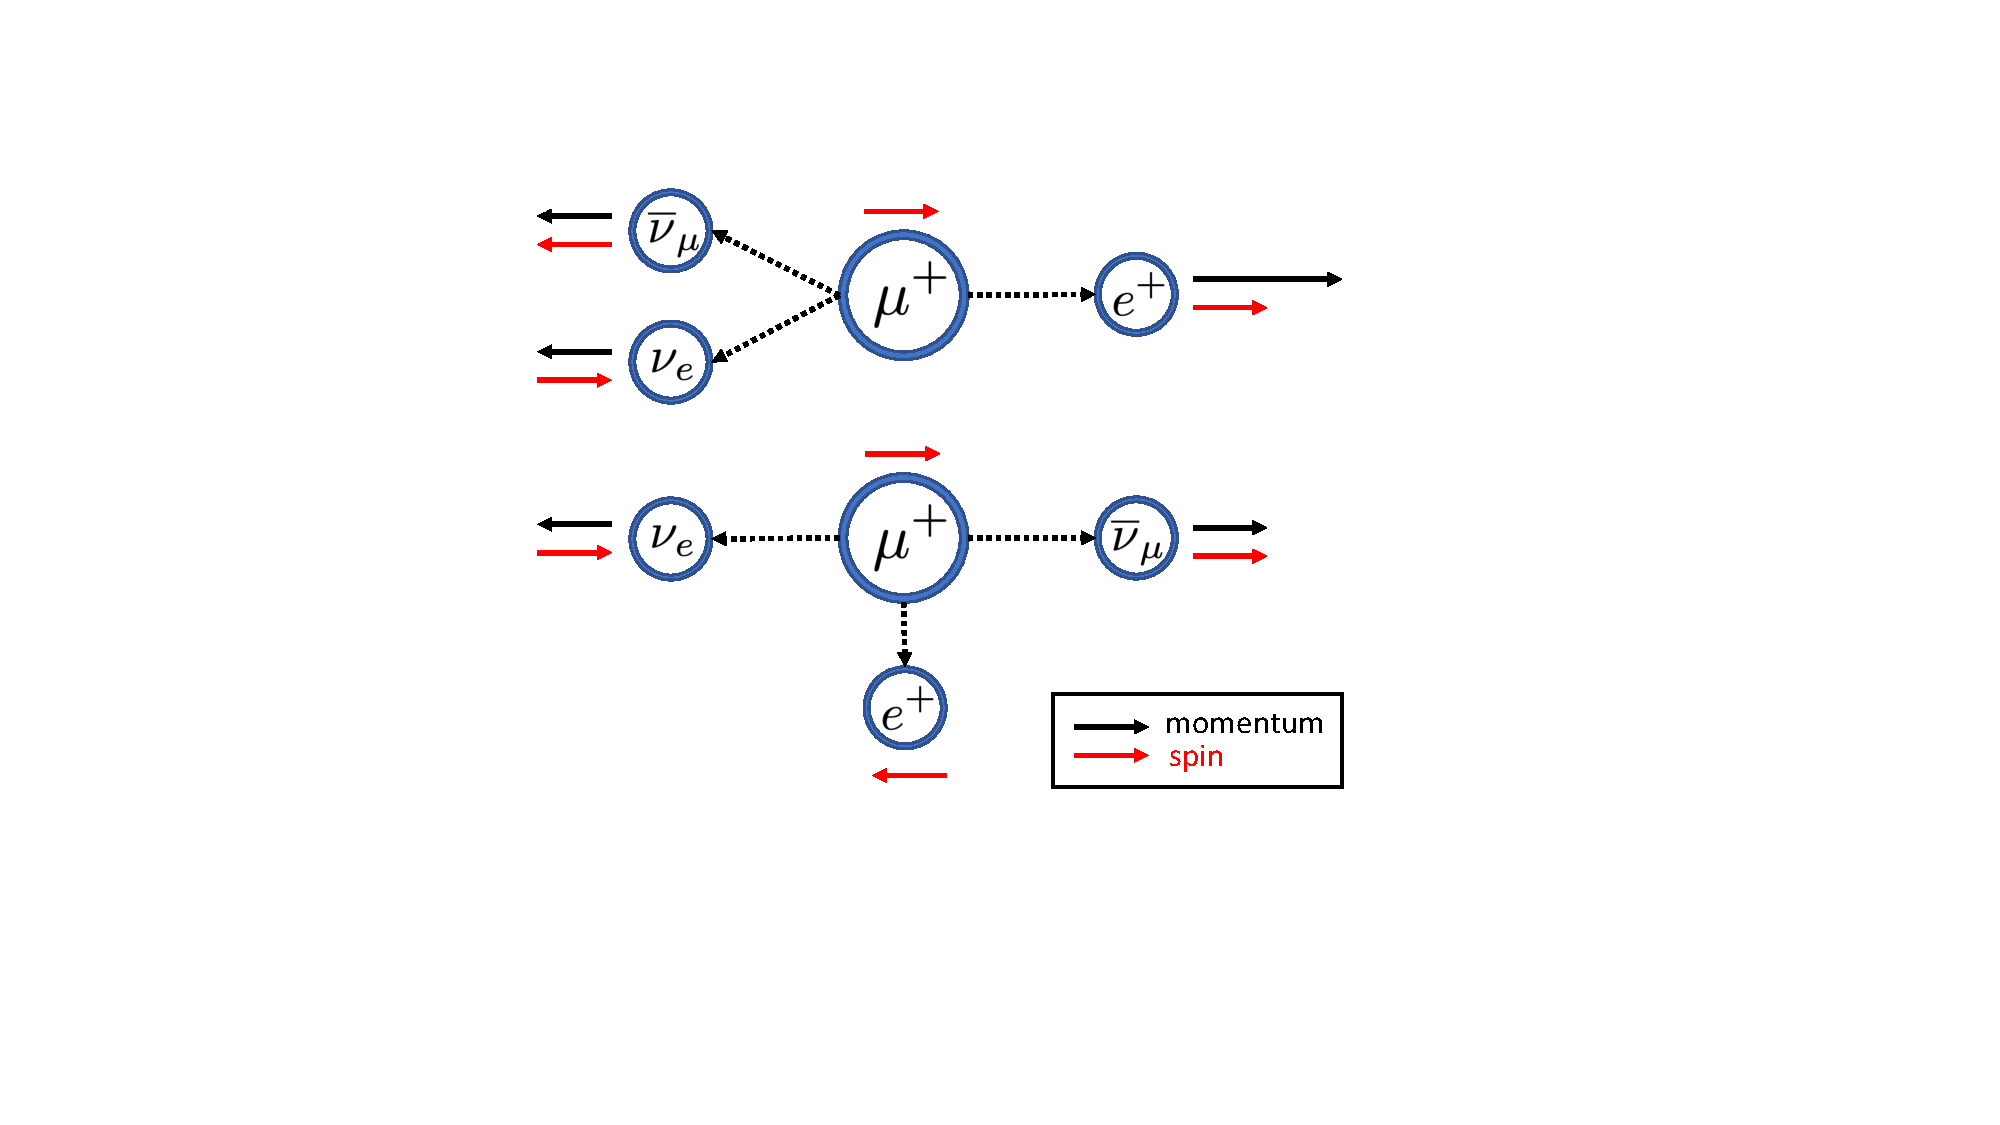
\includegraphics[width=0.6\textwidth]{MuonDecayImproved}
    \caption[Muon decay pictures for maximum and minimum energy decay positrons]{Muon decay pictures for maximum and minimum energy decay positrons. Due to the conservation of angular momentum and the single possible helicity states of the decay neutrinos, the spin of the decay positron is exactly parallel to the spin of the muon at the time of the decay for maximum energy decay positrons (top), or anti-parallel for minimum energy decay positrons (bottom).}
    \label{fig:MuonDecayImproved}
\end{figure}


This correlation between the emitted direction of the decay positron and the spin of the muon is the signature needed to measure \wa. By placing an ensemble of polarized muons within a magnetic storage ring, those muons will orbit at the cyclotron frequency and their spins will precess at the Larmour frequency. As they go around the ring they will decay to positrons whose energy and decay directions contain information about the spin of the muon. The differential decay distribution in the muon rest frame is described by \cite{Bucksbaum}
        \begin{align} \label{eq:diffdecaydist}
            dP(y, \theta) \propto N(y)[1 \pm A(y)\cos(\theta)]dy d\Omega,
        \end{align}
where $y=E/E_{max}$ is the energy fraction of the positron, $\theta$ is the angle between the spin of the muon and the momentum of the positron $\cos^{-1}(\hat{p} \cdot \hat{s})$, and the $\pm$ stands for the positive and negative muon respectively. $N(y)$ is the number distribution of decay positrons and $A(y)$ is the so called 'asymmetry' encoding the preferred positron decay direction. Here the energy of the positron is assumed to be much greater than its mass. The number distribution and asymmetry are given by \cite{Bucksbaum}
        \begin{align}
            N(y) &= 2y^{2}(3-2y^{2}), \label{eq:Nmrf} \\
            A(y) &= \frac{2y-1}{3-2y}, \label{eq:Amrf}
        \end{align}
and are shown in \figref{fig:NA2mrf}. 

\begin{figure}[]
\centering
    \begin{subfigure}[]{0.45\textwidth}
        \centering
        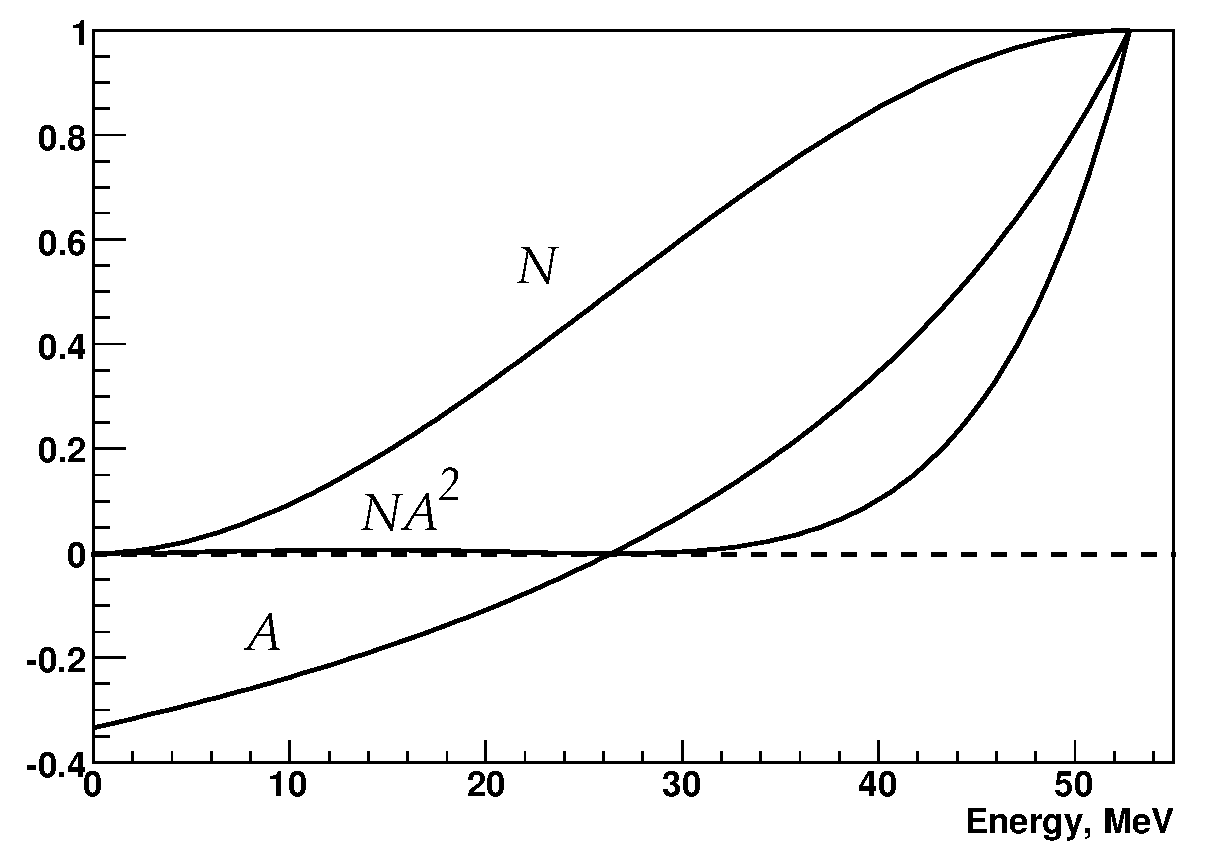
\includegraphics[width=\textwidth]{NA_mrf}
        \caption{Muon rest frame}
    \label{fig:NA2mrf}
    \end{subfigure}%
    \hspace{1cm}
    \begin{subfigure}[]{0.45\textwidth}
        \centering
        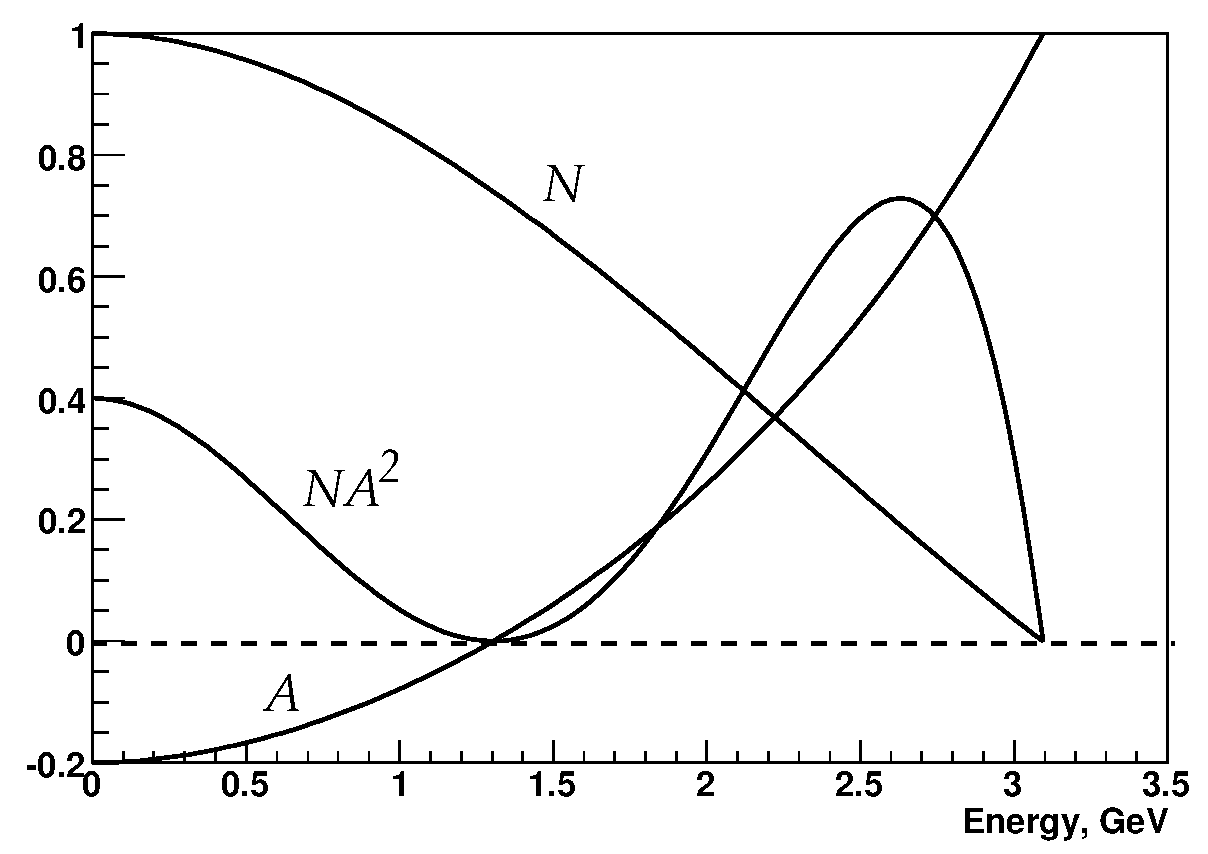
\includegraphics[width=\textwidth]{NA_lab}
        \caption{Lab frame}
    \label{fig:NA2lab}    
    \end{subfigure}
\caption[Number distribution and asymmetry for muon decay in the muon rest frame and lab frame]{Decay number distribution $N$ and asymmetry $A$ in the muon rest frame (left) and in the lab frame (right) as a function of positron energy with a maximum positron energy of 3.1 \GeV.}
\label{fig:NA2}
\end{figure}

In the lab frame for high energy positrons, nearly all positrons will be emitted parallel to the muon momentum, which makes it challenging to select purely on the decay angle of the positron. That's not a problem though, as we already know that decay positrons with higher energies will be emitted in directions parallel to the muon spin at the time of decay. Essentially, the energy distribution of detected positrons for high energies is modulated by \wa, or $\theta = \omega_{a}t + \phi$. The number of detected positrons at some time and energy in the lab frame for some initial number $N_{0}$ of muons can then be described by
        \begin{align}
            N_{d}(t, E) = N_{0}(E) \cdot e^{-t/\gamma\tau_{\mu}} \cdot [1 + A(E) \cos(\omega_{a}t+\phi(E))],
        \end{align}
where the $d$ subscript stands for 'detected,' the muons are decaying at a lifetime of $\gamma\tau_{\mu}$, and all the relevant parameters are energy dependent. Here $N_{0}(E)$ and $A(E)$ have been transformed from Equations~\ref{eq:Nmrf} and \ref{eq:Amrf} to the lab frame,
        \begin{align}
            N_{0}(E) &\propto (y-1)(4y^{2}-5y-5), \label{eq:Nlab} \\
            A(E) &= \frac{-8y^{2}+y+1}{4y^{2}-5y-5}, \label{eq:Alab}
        \end{align}
where as a reminder $y=E/E_{max}$. Here the polarization of the muons is assumed to be unity. These are shown in \figref{fig:NA2lab}. To increase the amount of statistics, all positrons above some energy threshold cut $E_{th}$ can be taken as the observable,
        \begin{align} \label{eq:5parfunc}
            N_{d}(t, E_{th}) = N_{0}(E_{th}) \cdot e^{-t/\gamma\tau_{\mu}} \cdot [1 + A(E_{th}) \cos(\omega_{a}t+\phi(E_{th}))],
        \end{align}
where the number and asymmetry of the detected positrons is now calculated by simply integrating Equations~\ref{eq:Nlab} and \ref{eq:Alab} from $y_{th}$ to 1,
        \begin{align}
            N_{0}(E_{th}) &\propto (y_{th}-1)^{2}(-y_{th}^{2}+y_{th}+3), \label{eq:Nth} \\
            A(E_{th}) &= \frac{y_{th}(2y_{th}+1)}{-y_{th}^{2}+y_{th}+3}, \label{eq:Ath}
        \end{align}
where $y_{th}=E_{th}/E_{max}$. By fitting \equref{eq:5parfunc}, \wa can be extracted. An sample of data adhering to \equref{eq:5parfunc} is shown in \figref{fig:gm2wiggle}.


\begin{figure}[]
    \centering
    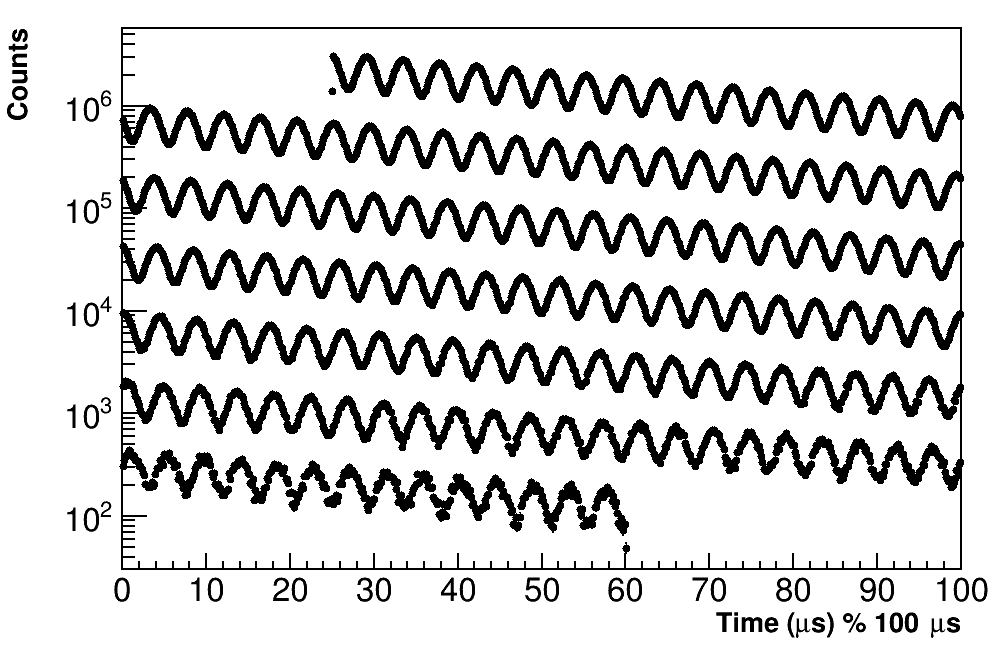
\includegraphics[width=0.9\textwidth]{gm2wiggle}
    \caption[\gmtwo wiggle example]{The number of detected positrons above some energy threshold ($y \sim 0.55$) as a function of time. The time axis is wrapped around every \mus{100}.}
    \label{fig:gm2wiggle}
\end{figure}



\section{Measuring the magnetic field}
\label{sec:BIntro}


In order to measure the magnetic moment of the muon to 140 ppb, the field needs to be both highly uniform, and measured to extreme precision. 



in \equref{fig:MagnetCrossSection}

\begin{figure}[]
    \centering
    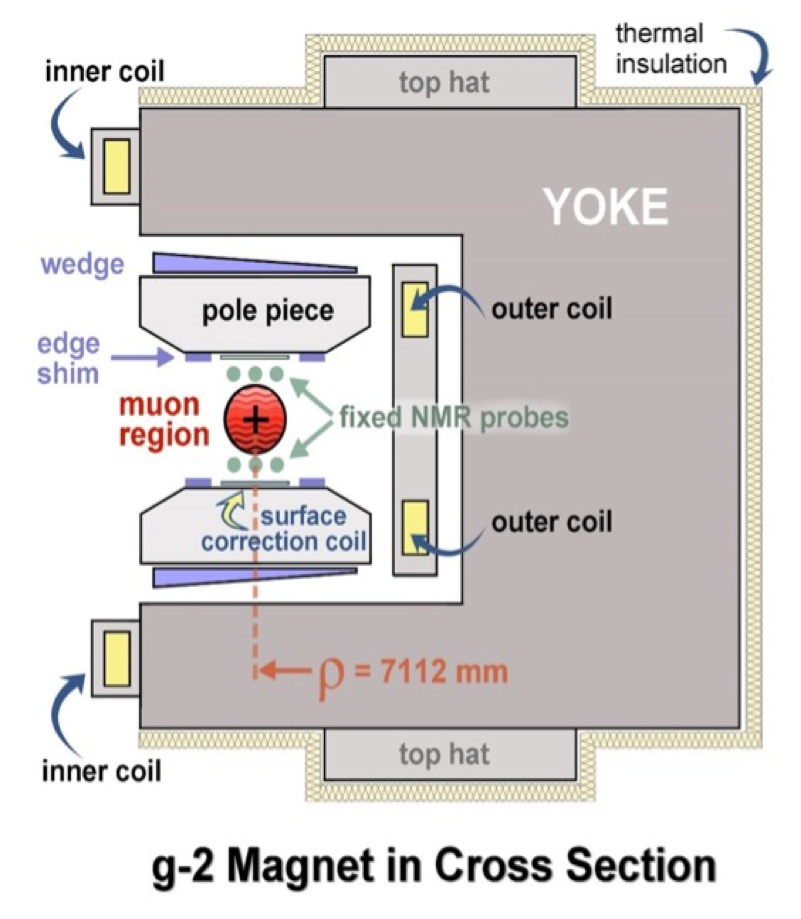
\includegraphics[width=0.9\textwidth]{MagnetCrossSection}
    \caption[Magnet cross section]{captuoin}
    \label{fig:MagnetCrossSection}
\end{figure}



Measuring the magnetic field boils down to measuring $\omega_{p}$ as shown in \equref{eq:wp}. This is because the magnetic field measurement is made using a pulsed nuclear magnetic resonance technique (NMR). NMR probes work by rotating the magnetization of a sample of protons in some fluid, typically water or petroleum jelly, and then measuring the relaxation time or free-induction decay (FID) signal of the proton spins. The magnetization of the protons will relax back to zero as the spins of the protons precess at the Larmour frequency and interact with local magnetic field gradients or inhomogeneities. Pickup coils are located around the sample which both deliver the pulse to rotate the proton sample magnetization and measure the FID signal. An example of an FID signal is shown in \figref{fig:FID}.

\begin{figure}[]
    \centering
    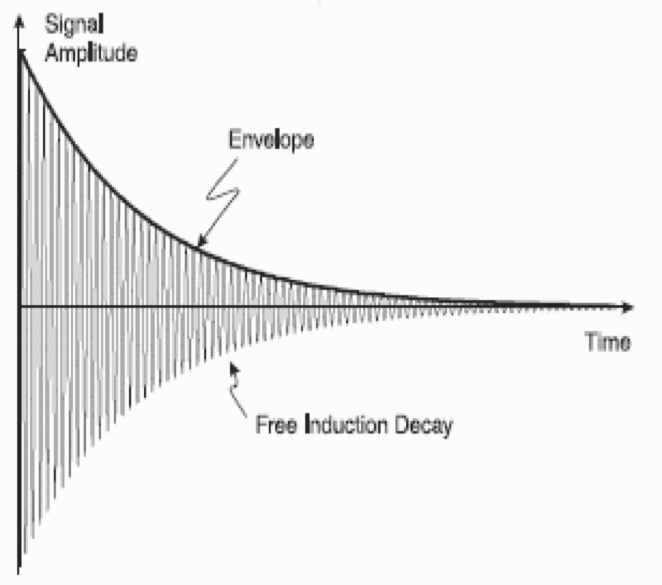
\includegraphics[width=0.6\textwidth]{FID}
    \caption[FID signal]{An example FID signal. The current picked up in the coils around the proton sample will oscillate as the spins precess around the main magnetic field, and decay as the spins return to alignment with the external field.}
    \label{fig:FID}
\end{figure}

Technically, it is not solely $\omega_{p}$ that needs to be measured. What really matters is the average magnetic field that the muons see, or the time-averaged spatially-weighted magnetic field. The scheme devised to measure this is two-fold. First, the magnetic field in the storge region where the muons live is measured by a trolley which drives around the inside of the ring. This trolley holds 17 NMR probes and measures the field at approximately 6000 locations around the inside of the ring. Because however the trolley cannot be in the beam path when the muons are present in the ring, it is pulled out of the way and the field is instead measured by 378 fixed NMR probes located in the high magnetic field region but just outside the storage region. The prescription is that the fixed probes measure the field at all times, the storage ring field is measured every few days by the trolley probes, and the two are interpolated. In this way the magnetic field can be mapped over time and over the space that the muons live in. A preliminary sample of the azimuthally-averaged magnetic field measured with trolley and fixed probes is shown in \figref{fig:AverageMagneticField}. (Might want to find a better picture, and also figure out what the time averaging is. Also what is with the vertical and radial width of the measured field?)

\begin{figure}[]
    \centering
    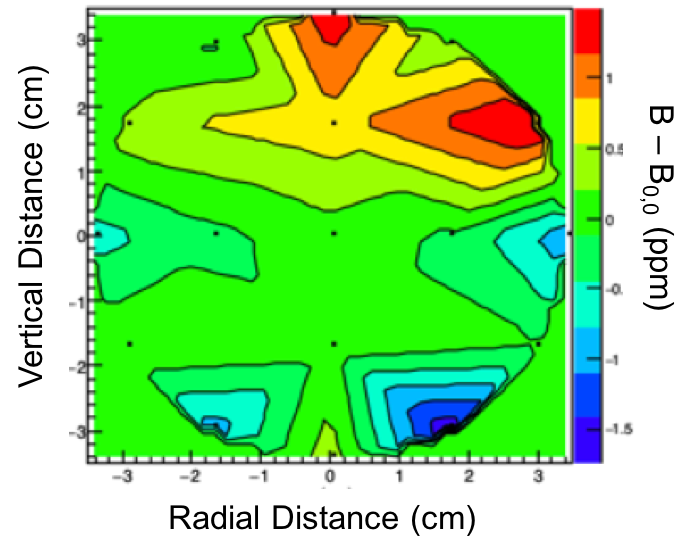
\includegraphics[width=0.6\textwidth]{AverageMagneticField}
    \caption[Azimuthally averaged magnetic field sample]{A sample of the azimuthally-averaged magnetic field within the storage region. The contours are normalized to the center value of the field. The scale of the field differences is approximately $\pm 1$ ppm. The dots in the picture correspond to the location of the trolley probes.}
    \label{fig:AverageMagneticField}
\end{figure}


The other half of the experiment is measuring the magnetic field ...



Technically wp should be ...
Finally, the magnetic field that needs to be measured is the magnetic field that the 


Very uniform field...


Finally the measurement of the field needs to be calibrated...







\section{Storage of muons and corrections to \texorpdfstring{\wa}{wa}}
\label{section:WaIntro}




\clearpage





In the presence of an electric field, which is useful in storing the muon beam within a dipole magnetic field, this expands to 
        \begin{align} \label{eq:waelectric}
            \vec{\omega}_{a} = -\frac{Qe}{m} [a_{\mu}\vec{B} - (a_{\mu} - \frac{1}{\gamma^{2}-1})(\vec{\beta} \times \vec{E}) ],
        \end{align}
where now the measurable quanties are vector quantities. Finally, for realistic cases of muon momentum which is non-orthogonal to the magnetic field, the spin difference frequency becomes
        \begin{align} \label{eq:wafinal}
            \vec{\omega}_{a} = -\frac{Qe}{m} [a_{\mu}\vec{B} - a_{\mu} (\frac{\gamma}{\gamma+1})(\vec{\beta} \cdot \vec{B})\vec{B} - (a_{\mu} - \frac{1}{\gamma^{2}-1})(\vec{\beta} \times \vec{E}) ].
        \end{align}
If the motion of the muons is largely perpendicular to the magnetic field, then the second term is small and can be corrected for. If the particles have a momentum of approximately 3.09 \GeV/c, the so called ``magic momentum,'' then the third term is small and can be corrected for. These will be talked about later.

In order to measure the spin difference frequency of the muon, a clever technique is used. Decay muons in the pion rest frame are 100\% polarized due to conservation of angular momentum and the fact that the decay neutrino must have a specific helicity. Within a pion beam then the highest and lowest energy decay muons are polarized. Muons will decay to positrons with a lifetime of about 2.2 $\mu$s, and the positrons with the highest energies will be correlated with the muon spin, a so called ``self-analyzing'' decay. The single available decay state for a maximum energy positron illustrates this in \figref{fig:MuonDecay}. Thus, by aquiring a large sample of polarized muons and injecting them into a storage ring 







\begin{figure}[]
    \centering
    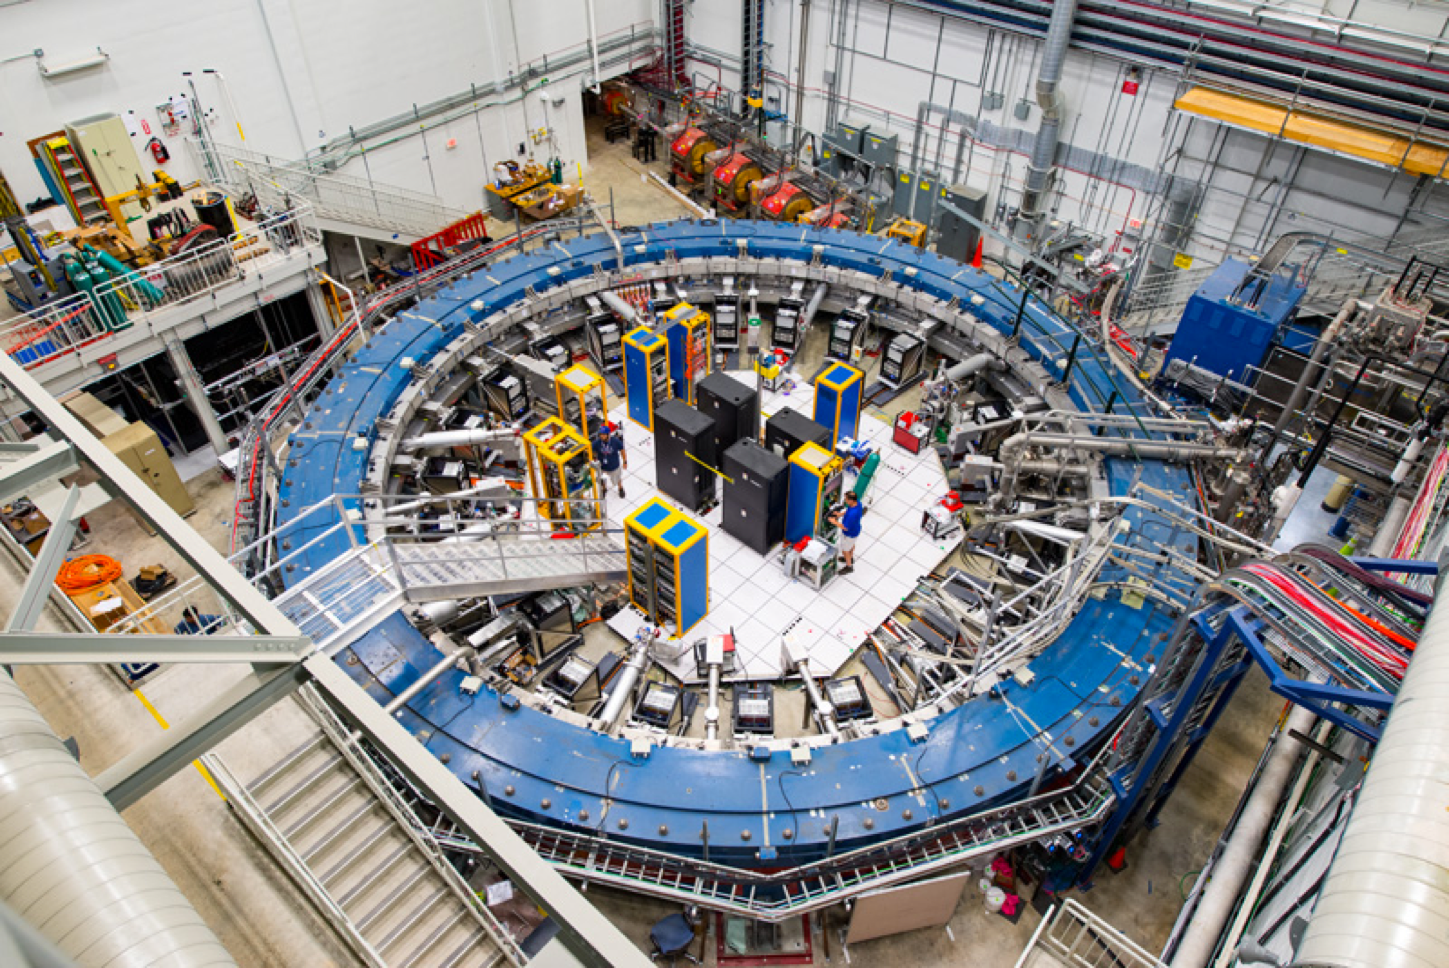
\includegraphics[width=0.9\textwidth]{ring}
    \caption[ring]{clean up and possibly replace}   
    \label{fig:ring}
\end{figure}












\section{Accelerator}
\label{sec:Accelerator}




\cite{Stratakis:2017uci}


\section{Injection}
\label{sec:Injection}

the inflector



\section{Storage}
\label{sec:Storage}

kickers and quads




